%!TEX root =  karen.tex


\chapter{Introduction}


\subsubsection{Background on GPUs} 

GPUs were introduced in 80's \hl{see master's thesis}.

Originally GPUs were designed as parallel rasterizing units. They had limited logic control in contrast to the serial CPUs and their advanced branching and looping logic. 

Gradually new and complex logic was added to the GPU to produce the shader languages that allowed developers to customize specific parts of the rendering pipeline. This allowed scientific problems such as the diffusion equation \hl{cite Lore and others} to be solved in process of rendering. In other words, the GPU was tricked into computing.

The year 2006 brought the modern age of GPU computing with the introduction of CUDA from NVidia. The high level language allowed scientists to leverage the GPU as a parallel accelerator without all of the overhead of setting up graphics contexts and tricking the hardware into computing. Memory management is still the developer's responsibility, but compiler transforms generic C/Fortran code to GPU instruction set. 

Scientific Computing has seen a widespread adoption of GPGPU because of the goal to get to ``exa-scale'' computing, which may only be possible in the near future with the help of GPU accelerators \cite{GPUandExascale2011}. 

NVidia is not the only company involved in many core parallel accelerators. Other groups like AMD and Intel have been increasing the number of cores as well. The end effect is a hybridization where CPUs look similar to GPUs and vice-versa. 

Until 2009, the hardware distinction required that developers target parallelism on CPUs and GPUs using different languages. Then the OpenCL standard was drafted and implemented. OpenCL is a parallel language that strives to provide functional portability rather than performance. 

We focus on the OpenCL language within this dissertation with confidence that hardware will change frequently. In fact, every 18 months \hl{cite} shows a new release of GPU hardware, manycore CPU hardware and extensions to parallel languages. But if hardware is constantly changing, then we need to focus on a high level implementation that allows portability. We need a language like OpenCL to carry our implementations into the future regardless of what hardware and which company survive. 

\subsubsection{Scientific problems and the need for computational methods} 

Many scientific problems of importance can be expressed as a collection of partial differential equations defined for some domain. In order to solve these 
problems , computational numerical methods are employed on a discretized version of the domain. Traditionally, three major categories exist for PDE solutions: \hl{ finite difference (FD), finite element (FEM) and spectral element (SEM)} \cite{Fasshauer:2007}. Interestingly, all three of these methods rely on an underlying mesh, making them \emph{meshed methods}. While each has had a turn in the spotlight, more recently a new category, or rather a generalization on all three previous categories, has emerged: \emph{meshfree methods}. 

\subsubsection{Traditional methods (FD, FV, FEM, SEM) and their dependence on structured meshes and ``nice'' connections (e.g., Delaunay).}
Note, finite element allows for triangle meshes, but well balanced Delaunay are preferred to limit ill conditioning. The same regularity in nodes is preferred with RBF methods. The reason for this is to keep best conditioning of the system. 

Leaders in computational science are cobbled together with metaphorical bubble gum and duct tape. Many scientists neglect to plan in advance for items like: 
\begin{itemize}
\item generic point clouds; most methods require a point cloud include some connectivity information for structured and unstructured mesh. 
\item we need to add adaptive mesh refinement
\item we need to avoid pole singularities
\item save on interpolations and differences but get similar answer in O($nm$). 
\end{itemize} 

\subsubsection{ recently, meshfree methods surfaced leveraging RBFs}

\subsubsection{ RBFs have interesting history. Started with interpolation, but went to collocation with global SEM scheme. The global scheme has $O(N^{2})$ complexity.}

\subsubsection{Most recently RBFs went to RBF-FD. Introduces sparsity and reduces cost of scaling.}


\subsubsection{For RBF problems in general there is limited work that scales the methods to large problems.}


\subsubsection{Large problems require high performance computing. Given lack of scaling in literature, it has been irrelevant until recently to assess the possibility of solving PDEs with RBF-FD on GPUs.}

\subsubsection{what is new in the thesis (summarize: 1-2 pages)}

The large scale contributions of this thesis can be summarized as follows: 
\begin{itemize} 
\item This thesis covers details related to the application of the RBF-FD method for both explicit and implicit solutions for PDES. 
\item Our domain decomposition algorithm provides the first known parallelization of RBF-FD across multiple CPUs.
\item Furthermore, we offload intense computational tasks to the GPU creating the first ever single- and multi-GPU implementation of RBF-FD. 
\end{itemize}
As part of the research on RBF-FD within those three areas we additionally contributed the following: 
\begin{itemize} 
\item Application of RBF-FD to Centroidal Voronoi Tessellation grids. 
\item Approximate Nearest Neighbor methods for faster neighbor queries and improved system conditioning
\item Multi-GPU implementations of sparse iterative Krylov solvers
\end{itemize} 


\subsubsection{Research Statement} 
What motivated this research?
\label{sec:intro}

The goal of this dissertation is to present a unified approach
to parallel solutions of Partial Differential Equations (PDEs)
with a method called Radial Basis Function-generated Finite
Differences (RBF-FD).

\hl{fix:}
Many scientific problems of importance can be expressed as a
collection of PDEs. Solutions to these problems provide answers to many simple
questions such as the current temperature of a material, or perhaps the
current position of a moving object. Complex and coupled PDEs can simulate the growth of zebra stripes or cheetah spots \cite{FuselierWright2012} or even model the flow of fluids. \hl{Need refs for examples}


In order to solve these problems, computational numerical
methods are employed on a discretized version of the domain.
Traditionally, three \hl{(and how would I classify FV? PartOfUnity?)} major categories exist for PDE solutions:
finite difference (FD), finite element (FEM) and spectral
element (SEM) \cite{Fasshauer2007}. Interestingly, all three of
these methods rely on an underlying mesh, making them
\emph{meshed methods}. While each has had a turn in the
spotlight, more recently a new category, or rather a
generalization on all three previous categories, has emerged:
\emph{meshfree methods}.

The first task in traditional meshed methods is to generate an
underlying grid/mesh. Node placement can be done in a variety of
ways including uniform, non-uniform and random (monte carlo)
sampling, or through iterative methods like Lloyd's algorithm
that generate a regularized sampling of the domain (see e.g.,
\cite{Du1999}). \hl{meshed methods have constraints on edge length and angle. Delaunay answers this, but is costly to compute}
\hl{Mesh2d, Triangle, DIstmesh} In addition to choosing nodes, meshed methods
require connectivity/adjacency lists to form stencils (FD) or
elements (FEM, SEM)---this implies an added challenge to cover
the domain closure with a chosen element type. While these tasks
may be straightforward in one- or two-dimensions, the extension
into higher dimensions becomes increasingly more cumbersome
\cite{Li2007}. 

Complex geometries, irregular boundaries and mesh refinement also pose a problem for meshed methods. As the complexity of 
the geometry/boundaries increases, so too should the resolution of the approximating mesh in order to 
accurately reconstruct the detail present. A na\"{i}ve approach to refinement increases the density of nodes uniformly across the 
domain, adding much more computation and memory storage than necessary for activity that is localized to sub-regions 
of the domain. Multiresolution methods attempt to compromise between accurate approximation of the domain and 
reduced resolution by one of two approaches: a) \emph{multilevel methods} that decompose the model into a hierarchy with 
several levels of mesh detail, then only use a level when it is required to capture phenomena; and b) \emph{adaptive irregular 
sampling} which has one level of detail, but non-uniform nodal density concentrated in areas of high activity \cite
{Iske2004}. Such techniques require robust methods and complex code capable of either coarsening/smoothing the 
approximate solutions to new level, or handling non-uniform node placement, element size etc. 

Ideally, we seek a method defined on arbitrary geometries, that behaves regularly in any dimension, and avoids the cost of 
mesh generation. The ability to locally refine areas of interest in a practical fashion is also desirable. Fortunately, meshfree 
methods provide all of these properties: based wholly on a set of independent points in $n$-dimensional space, 
there is minimal cost for mesh generation, and refinement is as simple as adding new points where 
they are needed. 

Since their adoption by the mathematics community in the 1980s (\cite{Fasshauer2007}), a plethora of meshfree methods have 
arisen for the solution of PDEs. For example, smoothed particle hydrodynamics, partition of unity method, element-free Galerkin 
method and others have been considered for fluid flow problems \cite{Chandhini2007}. For a recent survey of methods see \cite{Li2007}.


A subset of meshfree methods of particular interest to the
community today revolves around Radial Basis Functions (RBFs).
RBFs are a class of radially symmetric functions (i.e.,
symmetric about a point, $x_j$, called the \emph{center}) of the
form: 
	\begin{equation} 
		\phi_j(\vx) = \phi(r(\vx))
	\end{equation} 
where the value of the univariate function $\phi$ is a
function of the Euclidean distance from the center point $\vx_j$ given by
$r(\vx) = ||\vx-\vx_j||_2 = \sqrt{(x-x_j)^2 + (y-y_j)^2 + (z-z_j)^2}$. Examples of
commonly used RBFs are available in \hl{Table}~\ref{tbl:rbfs}
with their corresponding plots in Figure~\ref{fig:rbfs}. RBF
methods are based on a superposition of translates of these
radially symmetric functions, providing a linearly independent
but non-orthogonal basis used to interpolate between nodes in
$n$-dimensional space. An example of RBF interpolation in 2D
using 15 Gaussians is shown in
Figure~\ref{fig:rbfInterpolation}, where $\phi_j(r(\vx))$ is an
RBF centered at $\{\vx_j\}_{j=1}^{n}$.

\begin{figure}[ht]
\centering
	\begin{subfigure}[b]{0.25\textwidth}
    	\centering
		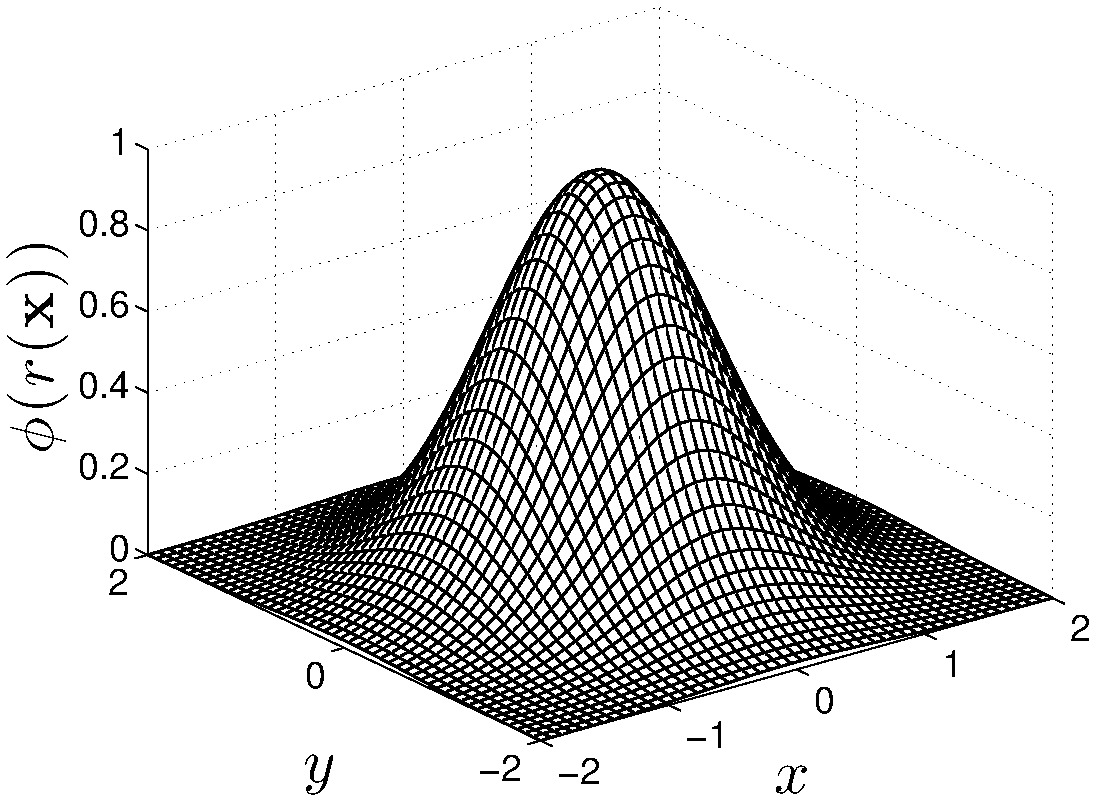
\includegraphics[width=1.0\textwidth]{figures/paper1/figures/ga_rbf2d-eps-converted-to.pdf} 
		\caption{Gaussian}
	\end{subfigure}
	\begin{subfigure}[b]{0.25\textwidth}
	\centering
		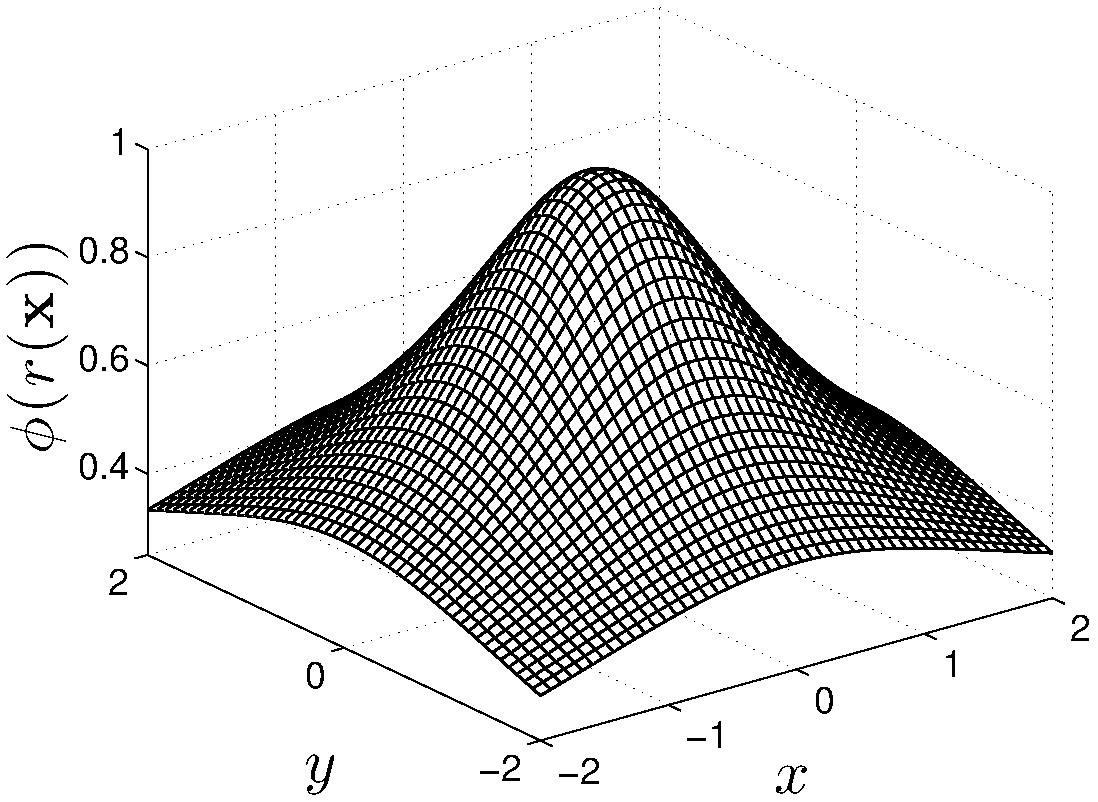
\includegraphics[width=1.0\textwidth]{figures/paper1/figures/imq_rbf2d-eps-converted-to.pdf}
		\caption{Inverse Multiquadric}
	\end{subfigure}
	\begin{subfigure}[b]{0.25\textwidth}
	\centering
		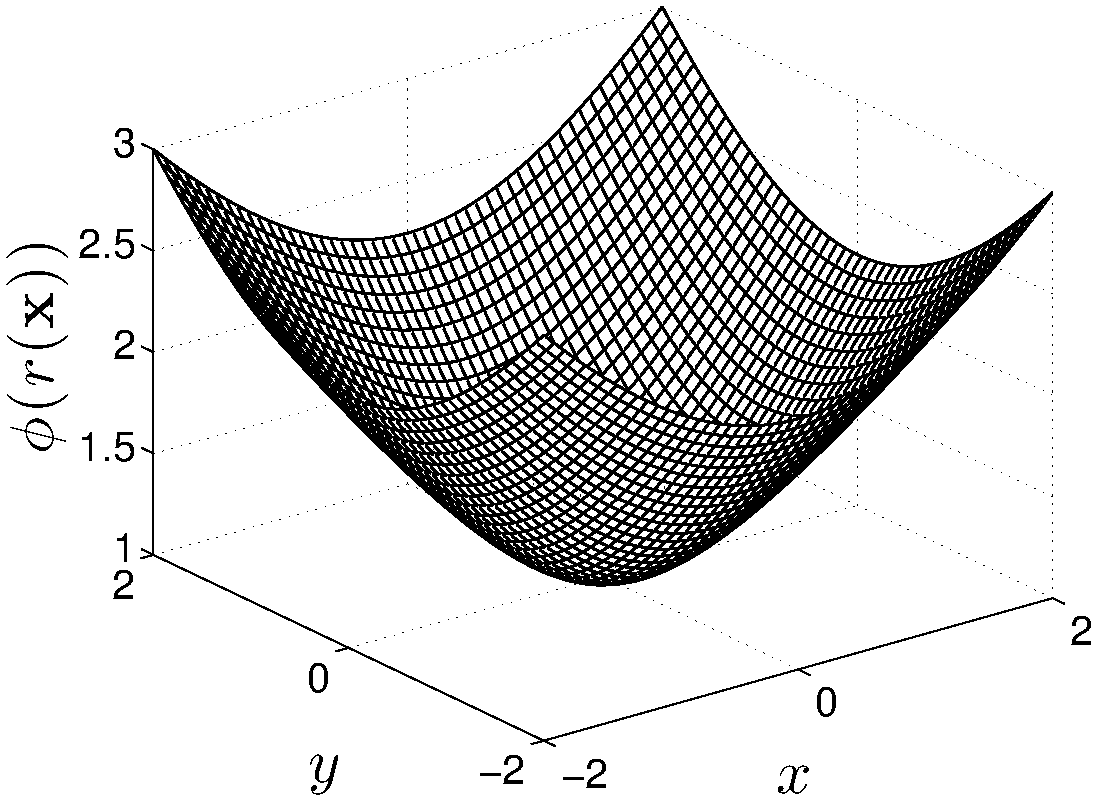
\includegraphics[width=1.0\textwidth]{figures/paper1/figures/mq_rbf2d-eps-converted-to.pdf} 
		\caption{Multiquadric}
	\end{subfigure} 
    \caption{Commonly used RBFs.}
    \label{fig:rbfs}
\end{figure}

%Numerical methods based on radial basis functions (RBFs) are rapidly gaining popularity for the solution of partial differential equations (PDEs). 
With a history extending back four decades for RBF interpolation schemes \cite{Hardy1971}, and two decades for RBFs applied to solving PDEs \cite{Kansa1990a}, many avenues of research remain untouched within their realm. Being a meshless method, RBF methods excel at solving problems that require geometric flexibility with scattered node layouts in $n$-dimensional space. They naturally extend into higher dimensions without significant increase in programming complexity \cite{FlyerWright07,WrightFlyerYuen10}. In addition to competitive accuracy and convergence compared with other state-of-the-art methods \cite{FlyerWright07, FlyerWright09, FlyerLehto10, WrightFlyerYuen10, FlyerFornberg11}, they also boast stability for large time steps.

Like most numerical methods, RBFs come with certain
limitations. For example, RBF interpolation is---in general---not a well-posed
problem, so it requires careful choice of positive definite or conditionally
positive definite basis functions \cite{Iske2004,Fasshauer2007}. 
The example 2D RBFs presented in Figure~\ref{fig:rbfs} are infinitely smooth and satisfy the (conditional) positive definite requirements. 

Infinitely smooth RBFs depend on a shape or support parameter $\epsilon$ that controls the width of the function. The functional form of the shape function becomes $\phi(\epsilon r)$. Decreasing $\epsilon$ increases the support of the RBF and in most cases, the accuracy of the interpolation, but worsens the conditioning of the RBF interpolation problem \cite{Schaback1995}. The \hl{conditioning} of the system also dramatically \hl{decreases} as the number of nodes in the problem increases. Fortunately, recent algorithms such as Contour-Pad\'{e} \cite{Fornberg2004} and RBF-QR \cite{Fornberg2007, Fornberg2011a} allow for numerically stable computation of interpolants in the nearly flat RBF regime (i.e., $\epsilon \rightarrow 0$) where high accuracy has been observed \cite{Larsson2003, Fornberg2008}.


Historically, the most common way to leverage RBFs for PDE solutions is in a global interpolation sense. That is, the value of a function value or any of its derivatives 
at a node location is a linear combination of all the function values over the \textit{entire} domain, just as in a pseudospectral method. If using infinitely smooth RBFs, this leads to spectral (exponential) convergence of the RBF interpolant for smooth data \cite{Fornberg2005}. %(need reference 
As discussed in {\cite{FlyerWright09}}, global RBF methods 
require $O(N^3)$ floating point operations (FLOPs) in pre-processing, where $N$ is the total number of nodes, to assemble and solve a dense linear system for differentiation coefficients. The coefficients in turn are assembled into a dense Differentiation Matrix (DM) that is applied via matrix-vector multiply to compute derivatives at all $N$ nodes for a cost of $O(N^2)$ operations. \hl{assumes explicit scheme}



% 
%   require a 
%preprocessing stage, executed once, to assemble and solve a linear 
%system to produce differentiation matrices for a cost of $O(N^3)$ floating point operations (FLOPS),
%where $N$ is the total number of RBFs. 
%The differentiation matrix is dense and applied via matrix-vector multiplication to obtain approximation function derivatives at the RBF node centers. The cost 
%of derivative calculation is $O(N^2)$.


Alternatively, one can use RBF-generated finite differences (RBF-FD) to introduce sparse DMs (Note: for pure interpolation, compactly supported RBFs can also introduce sparse matrices \cite{Wendland1995}).
RBF-FD was first introduced by Tolstykh in 2000 \cite{Tolstykh2000}, 
but it was the simultaneous, yet independent,
efforts in \cite{Shu2003}, \cite{Tolstykh2003a}, \cite{Wright2003} and \cite{Cecil2004} that gave the method its real start. 
RBF-FD 
share advantages with global RBF methods, 
like the ability to function without an underlying mesh, easily extend to higher dimensions and afford large time steps; however spectral accuracy is lost. 
Some of the advantages of RBF-FD 
include high computational speed together with high-order accuracy
(6th to 10th order accuracy is common) and the opportunity 
for parallelization.

The RBF-FD method is similar in concept to classical 
finite-differences (FD): both methods approximate derivatives as a weighted sum of values at nodes within a nearby neighborhood. The two methods differ in that the underlying differentiation 
weights are exact for RBFs rather than polynomials. 

As in FD, increasing the stencil size $n$  increases the accuracy of the approximation.
Given $N$ total nodes in the domain (such as on the surface of a sphere), $N$ linear systems, each of size $n \times n$, are solved to calculate the differentiation weights. Since $n \ll N$, the RBF-FD preprocessing complexity is dominated by $O(N)$---much lower than for the global RBF method of $O(N^3)$---with derivative evaluations on the order of $O(nN) \implies O(N)$ FLOPs. 

\chapter{Related Work}

\section{  GPUS for explicit and implicit methods }



\section{  GPUS/RBF }

\cite{Schmidt2009a,Schmidt2009b}. Our paper \cite{BolligFlyerErlebacher2012} introduced the first implementation of RBF-FD to span multiple CPUs and multiple GPUs. 

\section{  RBF/Finite-Difference }

\subsection{Global RBF Method}

\subsection{RBF-FD}
RBF-FD have been successfully employed for a variety of problems including Hamilton-Jacobi equations \cite{Cecil2004}, convection-diffusion problems \cite{Chandhini2007, Stevens2009b},
incompressible Navier-Stokes equations \cite{Shu2003,Chinchapatnam2009}, transport on the sphere \cite{FornbergLehto11}, and the shallow water equations \cite{FlyerLehto11}.

\section{  Preconditioners }

Many preconditioners are based on physical properties of the domain, PDE and the spectral properties of the numerical method. 

\section{   Sparse matrix libraries }
\section{  Various GPU/based libraries }

\subsection{CUSP}

GMRES in CUSP is based on the Givens rotations for the Arnoldi process. 

\subsection{ViennaCL}

GMRES in ViennaCL is based on Householder reflections for the Arnoldi process. 

We opted to leverage the ViennaCL package in most of our implementations. 

\section{  Parallel implementations of RBF}

As $N$ grows larger, it behooves us to work on parallel architectures, be it CPUs or GPUs. With regard to the latter, there is some research on leveraging RBFs on GPUs in the fields of visualization \cite{Cuntz2007,Weiler2005},  surface reconstruction \cite{Corrigan2005,Carr2003}, and neural networks \cite{Brandstetter2008}. However, research on the parallelization of RBF algorithms to solve PDEs on multiple CPU/GPU architectures is essentially non-existent. We have found three studies that have addressed this topic, none of which implement RBF-FD but rather take the avenue of domain decomposition for global RBFs (similar to a spectral element approach). In \cite{Divo2007}, Divo and Kassab introduce subdomains with artificial boundaries that are processed independently. Their implementation was designed for a 36 node cluster, but benchmarks and scalability tests are not provided. Kosec and \v{S}arler \cite{Kosec2008} parallelize coupled heat transfer and fluid flow models using OpenMP on a single workstation with one dual-core processor. They achieved a speedup factor of 1.85x over serial execution, although there were
no results from scaling tests. Yokota, Barba and Knepley \cite{Yokota2010} apply a restrictive additive Schwarz domain decomposition to parallelize global RBF interpolation of more then 50 million nodes on 1024 CPU processors. Only Schmidt et al. \cite{Schmidt2009b} have accelerated a global RBF method for PDEs on the GPU. Their MATLAB implementation applies global RBFs to solve the linearized shallow water equations utilizing the AccelerEyes Jacket \cite{JacketGuide2009} library to target a single GPU.

\begin{figure}[t]
    \centering
    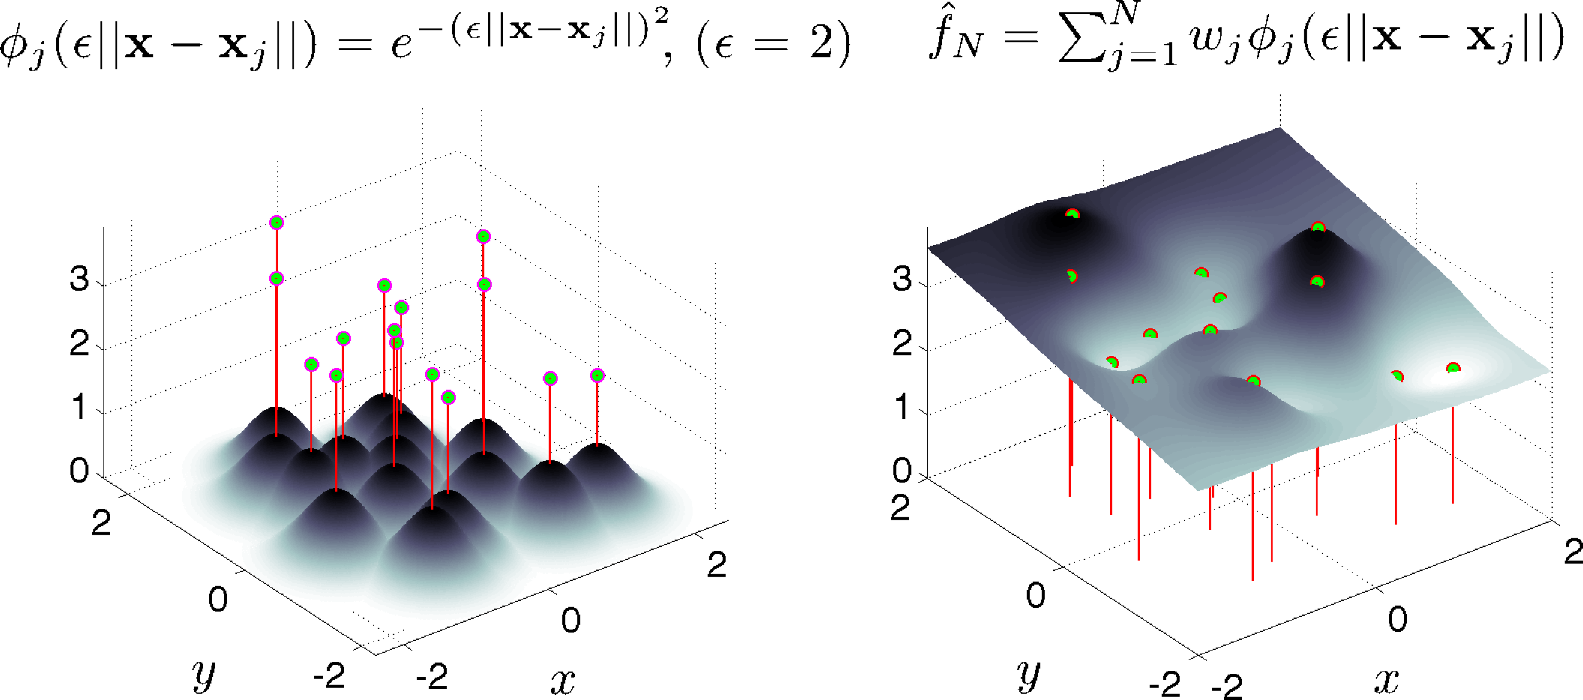
\includegraphics[scale=0.4]{figures/paper1/figures/trimmed_interpolate2D_ga__m.pdf}
    \caption{RBF interpolation using 15 translates of the Gaussian RBF with $\epsilon=2$. One RBF is centered at each node in the domain. Linear
    combinations of these produce an interpolant over the domain passing through known function values. }
    \label{fig:rbfInterpolation}
\end{figure}

\section{ Contributions of this Work }
%To our knowledge, this paper presents the first implementation of RBF-FD

Within this dissertation, we have developed the first implementation of RBF-FD
to span multiple CPUs. Each CPU has a corresponding GPU attached to it
in a one-to-one correspondence. We thus also introduced the first known 
implementation of accelerated RBF-FD on the GPU.

 \hl{continue with outline of chapters} 
We present our explicit and implicit solutions to PDEs with our multi-GPU RBF-FD implementation. 
%Within the scope of this paper we detail our method for spanning RBF-FD across multiple CPU/GPU processors and emphasize numerical validation of the implementation rather than optimization strategies. We will consider optimization in future work. The calculations are performed on Keeneland, a high performance computing installation supported by the National Science Foundation and located at Oak Ridge National Lab. Keeneland currently has 240 CPUs accompanied by 360 NVidia Fermi class GPUs with at least double that number expected by the end of 2012 \cite{Vetter2011}.

%The remainder of this paper is organized as follows:  Chapter~\ref{chap:rbffd} introduces RBF-FD via interpolation. Chapter~\ref{chap:gpu} details our parallelization strategies for the Keeneland system, including data partitions that are handled concurrently by different CPU processes and the data-parallel explicit time stepping scheme for the GPU. In Section~\ref{sec:validation}, our implementation is verified against well-known hyperbolic PDE test cases on the sphere, advection of a cosine bell and vortex wrap-up. Finally, performance benchmarks and results are presented in Section~\ref{sec:performance}, followed by conclusions and proposals for future optimization strategies in Section~\ref{sec:conclusion}.

\chapter{Fragments (integrate above) }

with the goal of solving coupled fluid flows modelling the physics (?) in the interior of the earth. We require both advective terms and diffusive terms. The components of a good pressure fluid solver are explicit and implicit differentiation. Whether we solve a steady-state PDE implicitly or a hyperbolic PDE with an implicit time-scheme, we require an \emph{implicit solver}. An implicit solver is nothing but a method of assembling a differentiation matrix, forcing terms on the RHS and then solving the linear system. A direct LU factorization would suffice if our system is dense, but with RBF-FD the system is sparse. Sparse systems can be efficiently solved under the right conditions through sparse iterative solvers. :


Sufficient understanding of RBF interpolation led to the development of the first global RBF method for PDEs in \cite{Kansa1990a}. Most popular among global methods is collocation, wherein RBF interpolation approximates the PDE solution by solving a large, dense linear system. 
In some cases RBF collocation demonstrates higher accuracy for the same number of nodes when compared to other state-of-the-art pseudospectral methods (e.g., \cite{Larsson2003} \cite{Flyer2007} \cite{Flyer2009b}). In \cite{Flyer2010}, spectral accuracy was demonstrated for hyperbolic PDEs even with local refinement of nodes in time.


Unfortunately---ill-conditioning aside---collocation methods are prohibitively expensive to solve when scaled to a large number of nodes. Assuming the collocation matrix does not change in time, global methods, with their dense systems, scale at $O(N^3)$ operations for initial preconditioning/preprocessing followed by $O(N^2)$ operations every time-step. This complexity is consistent with any collocation scheme. However, by introducing sparsity into the system (e.g., using compactly supported RBFs), the complexity is somewhat reduced.



General Purpose GPU (GPGPU) computing is one of today's hottest trends within scientific computing. 
The release of NVidia's CUDA at the end of 2006 marked both a 
redesign of GPU architecture, plus the addition of a new software layer that finally made GPGPU accessible to the general public. The CUDA API includes routines for memory control, interoperability with graphics contexts (i.e., 
OpenGL programs), and provides GPU implementation subsets of BLAS and FFTW libraries \cite{CudaGuide2011}. After the undeniable success of CUDA for C, new projects emerged to encourage GPU programming in languages like FORTRAN (see e.g., HMPP \cite{HMPP2009} and Portland Group Inc.'s CUDA-FORTRAN \cite{CudaFortran2009}). 

In early 2009, the Khronos Group--the group responsible for maintaining OpenGL--announced a new specification for a general 
parallel programming lanugage referred to as the Open Compute Language (OpenCL) \cite{OpenCL2009}. Similar in design to the CUDA language---in many ways it is a simple refactoring of the predecessor---the goal of OpenCL is to provide a mid-to-low level API and language to control any multi- or many-core processor in a uniform fashion. Today, OpenCL drivers exist for a variety of hardware including NVidia GPUs, AMD/ATI CPUs and GPUs, and Intel CPUs. 

This \textit{functional portability} is the cornerstone of the OpenCL language. However, functional portability does not imply performance portability. That is, OpenCL allows developers to write kernels capable of running on all types of target hardware, but optimizing kernels for one type of target (e.g., GPU) does not guarantee the kernel will run efficiently on another target (e.g., CPU).
% Already, today, CPUs are tending toward many core architectures. Simultaneously, the once specialized many-core GPUs now offer general purpose functionality. New architectures like the AMD Fusion \cite{AMDFusion} join CPU and GPU on the same chip proving that 
%, and It is easy to see that soon the CPU and GPU will meet somewhere in the middle as general purpose many-core architectures. OpenCL is an attempt to standardize programming before this intersection occurs. 
With CPUs tending toward many cores, and the once special purpose, many-core GPUs offering general purpose functionality, it is easy to see that soon the CPU and GPU will meet somewhere in the middle as general purpose many-core architectures. Already, ATI has introduced the Fusion APU (Accelerated Processing Unit) which couples an AMD CPU and ATI GPU within a single die. OpenCL is an attempt to standardize programming ahead of this intersection. 

%Home computers, smart-phones and other devices containing many- or multi-core compute units internally have driven the generalization of the accelerator language to provide a unified approach to targeting any available hardware. 

Petascale computing centers around the world are leveraging GPU accelerators to achieve peak performance. In fact, many of today's high performance computing installations boast significantly more GPU accelerators than CPU counterparts. The Keeneland project is one such example, currently with 240 CPUs accompanied by 360 NVidia Fermi class GPUs with at least double that number expected by the end of 2012 \cite{Vetter2011}. 

Such throughput oriented architectures require developers to decompose problems into thousands of independent parallel tasks in order to fully harness the capabilities of the hardware. To this end, a plethora of research has been dedicated to researching algorithms in all fields of computational science. Of interest to us are methods for atmospheric- and geo-sciences. 


\section{Fragments} 

\begin{verbatim}
- what is new in the thesis (summarize: 1-2 pages)
- get all your figues
- 1/2 page description per figures
  All figure captions (self-contained). Don't skimp on words.
- Previous work
  GPUS/implicit methods
  GPUS/RBF
  RBF/Finite-Difference
  Preconditionners (info on that)
   Sparse matrix libraries
  Various GPU/based libraries
   Parallel implementations of RBF (there are any?)

Benchmarking....
   Timing (serial, parallel)
   Timing with special node reorderings. Explain logic

Test cases ...

Get all your references in bibtex. Send them to me.


Need detailed table of content.
 \end{verbatim}		






As will be demonstrated in Chapter~\ref{chap:related}, most of the literature surrounding the solution of PDEs with RBFs is based on 
collocation. Collocation finds an interpolant that passes through a set of \emph{collocation points} (commonly chosen to coincide with RBF centers) satisfying the differential equations with zero residual. Collocation, then, is a global interpolation problem. Alternative methods exist based on local collocation formulations (see \cite{Sarler:2006, Vertnik:2006,Stevens:2008a, Stevens:2009a, Stevens:2009b}). Recently, an new approach using FD-like stencils to approximate 
differential operators was proposed  (see e.g., \cite{Wright:2003, Wright:2006, Shu:2003, Chandhini:2007}). The so-called RBF-FD method uses RBFs to interpolate initial conditions, but not the differential equations---generalized FD stencils approximate differential operators. 

Even today, RBFs are still up-and-coming in the scientific world with many avenues of research left to consider. Global formulations are understood to have spectral convergence properties, high accuracy and other benefits like adaptivity and ease of implementation over meshed methods \cite{Fasshauer:2007}. However, little is known about the behavior of local and RBF-FD methods. Open questions include (but are in no way limited to): a) ideal node placement to eliminate singularities; b) data-structures for stencil storage and evaluation; c) problem sizes larger than a few thousand nodes; and d) parallel implementations across new heterogeneous multi- and many-core architectures. In response to this, our group, in collaboration with researchers assembled from a national lab and four universities (see Chapter~\ref{chap:funding}), has been granted funds by the National Science Foundation to collaboratively:

\begin{quote}
\emph{``Bring RBFs to the forefront of multi-scale geophysical modeling by developing fast, efficient, and parallelizable RBF algorithms in arbitrary geometries, with performance enhanced by hardware accelerators, such as graphic processing units (GPUs)."} \cite{RBF_proposal:2009}
\end{quote}

In the last few years, GPUs transitioned from hardware dedicated to the embarrassingly parallel tasks involved in graphics rendering (e.g., 
rasterization) into multi-core co-processors for high performance scientific computing.  Thanks to the highly profitable and always demanding gaming industry, what began as a static rendering pipeline, was molded to allow fully dynamic execution with a SIMD-like programming model (Single Instruction Multiple Threads or SIMT). Changes in hardware were 
followed closely by evolving programming languages. Today, GPUs can be manipulated via high level 
languages 
similar to C/C++ and require no knowledge of computer graphics. 
In Chapters~\ref{chap:languages} and \ref{chap:hardware} we will discuss 
how GPU hardware and languages evolved to exceptionally higher compute capability than traditional CPUs, and became a popular platform for high performance computing.

True to our purpose statement above, the goal of this project is to integrate RBF methods for PDEs, Geophysics and large scale GPU computing. We begin in Chapter~\ref{chap:related} with a discussion of related work on RBF-PDE methods, their applications, and related work 
on GPUs. In Chapter~\ref{chap:rbf_pde} a formal introduction to RBFs for the solution of PDEs is provided. Chapter~\ref{chap:languages} considers various languages available for GPU computing and 
their appropriateness for our task. This is followed by a 
discussion in Chapter~\ref{chap:hardware} of GPU hardware and the large scale clusters with integrated GPUs which will be used for heterogeneous multi-core computing. Finally, in Chapter~\ref{chap:proposal} we present our proposal for research into efficient PDE 
solutions on multi-node, multi-GPU compute clusters using radial basis functions for Tsunami simulation.



